\begin{name}
	{\tenchude}
	{\tendethi}
	{Trường THPT Lê Thánh Tông TPHCM}
	{\thoigian}
\end{name}

\Opensolutionfile{ans}[ans/ans-2-TT-LeThanhTong]
%%==========Câu 1
\begin{ex}%[Dự án 16-TeamTeXHoa-THPT Lê Thánh Tông-Vũ Đức Hiếu]%[2D2Y5-1]%Câu 1
	Phương trình $\log_{3}(3x-2)=3$ có nghiệm là
	\choice
	{$x=\dfrac{25}{3}$}
	{$87$}
	{\True $\dfrac{29}{3}$}
	{$\dfrac{11}{3}$}
	\loigiai{
		$\log_{3}(3x-2)=3 \Leftrightarrow \heva{&3x-2>0\\&3x-2=3^3} \Leftrightarrow \heva{&x>\dfrac{2}{3}\\&x=\dfrac{29}{3}} \Leftrightarrow x=\dfrac{29}{3}$.
	} 
\end{ex}

%%==========Câu 2
\begin{ex}%[Dự án 16-TeamTeXHoa-THPT Lê Thánh Tông-Vũ Đức Hiếu]%[2H2B1-2]%Câu 2
	Cho hình nón có góc ở đỉnh bằng $120^\circ$ và diện tích xung quanh $2\pi\sqrt{3}$. Tìm chiều cao của hình nón.
	\choice
	{$\sqrt{2}$}
	{$\sqrt{3}$}
	{\True $1$}
	{$2$}
	\loigiai{
		\immini
		{Ta có $\widehat{BSA}=120^\circ \Rightarrow \widehat{ASO}=60^\circ$.\\
		Xét $\triangle SOA$ vuông tại $O$, có $\sin \widehat{ASO}=\dfrac{OA}{SA} \Rightarrow \dfrac{\sqrt{3}}{2}=\dfrac{OA}{SA} \Rightarrow OA=\dfrac{\sqrt{3}}{2}SA$.\\
		$S_{\text{xq}}=\pi OA\cdot SA \Rightarrow 2\pi\sqrt{3}=\pi\dfrac{\sqrt{3}}{2}SA^2 \Rightarrow SA=2 \Rightarrow OA=\sqrt{3}$.\\
		Vậy $SO=\sqrt{SA^2-OA^2}=1$.}
		{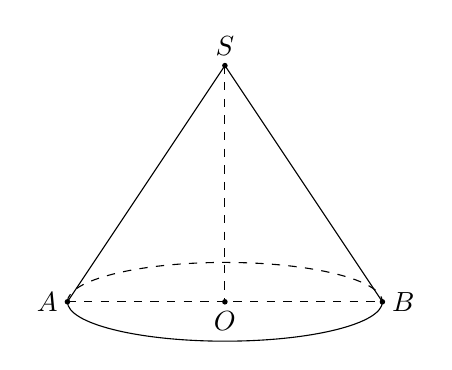
\begin{tikzpicture}
		\draw(0,0) arc(-180:0:{2} and {0.5});
		\draw[dashed](0,0) arc(180:0:{2} and {0.5});
		\coordinate [label=left:$A$](A) at(0,0);
		\coordinate [label=right:$B$](B) at(4,0);
		\coordinate [label=above:$S$](S) at(2,3);
		\coordinate [label=below:$O$](O) at(2,0);
		\foreach \point in {O,A,B,S} \fill[black](\point) circle(1pt);
		\draw(B)--(S)--(A);
		\draw[dashed](A)--(B)(S)--(O);
		\end{tikzpicture}}
	} 
\end{ex}

%%==========Câu 3
\begin{ex}%[Dự án 16-TeamTeXHoa-THPT Lê Thánh Tông-Vũ Đức Hiếu]%[2D1B2-1]%Câu 3
	Cho hàm số $y=f(x)$ có $f'(x)=x^2(x-1)^3(3-x)(x-5)$. Số điểm cực tiểu của hàm số là
	\choice
	{\True $1$}
	{$2$}
	{$3$}
	{$4$}
	\loigiai{
		Ta có $f'(x)=0 \Leftrightarrow x^2(x-1)^3(3-x)(x-5)=0 \Leftrightarrow \hoac{&x=0\\&x=3\\&x=5\\&x=1.}$\\
		Bảng biến thiên
		\begin{center}
			
\begin{tikzpicture}
				\tkzTabInit[nocadre,lgt=1.2,espcl=2.5,deltacl=0.6]
				{$x$/0.6,$y'$/0.6,$y$/2}
				{$-\infty$,$0$,$1$,$3$,$5$,$+\infty$}
				\tkzTabLine{,+,0,+,0,-,0,+,0,-}
				\tkzTabVar{-/$ $,R,+/$ $,-/$ $,+/$ $,-/$ $}
			\end{tikzpicture}
		\end{center}
		Dựa vào bảng biến thiên, số điểm cực tiểu của hàm số là $1$.		
	} 
\end{ex}

%%==========Câu 4
\begin{ex}%[Dự án 16-TeamTeXHoa-THPT Lê Thánh Tông-Vũ Đức Hiếu]%[2D3Y1-1]%Câu 4
	Cho $f(x)$, $g(x)$ là các hàm số xác định và liên tục trên $\mathbb{R}$. Trong các mệnh đề sau, mệnh đề nào \textbf{sai}?
	\choice
	{\True $\displaystyle\int f(x)g(x)\mathrm{\,d}x=\displaystyle\int f(x)\mathrm{\,d}x\cdot\displaystyle\int g(x)\mathrm{\,d}x$}
	{$\displaystyle\int{\left[f(x)+g(x)\right]}\mathrm{\,d}x=\displaystyle\int f(x)\mathrm{\,d}x+\displaystyle\int g(x)\mathrm{\,d}x$}
	{$\displaystyle\int{\left[f(x)-g(x)\right]}\mathrm{\,d}x=\displaystyle\int f(x)\mathrm{\,d}x-\displaystyle\int g(x)\mathrm{\,d}x$}
	{$\displaystyle\int 2f(x)\mathrm{\,d}x=2\displaystyle\int f(x)\mathrm{\,d}x$}
	\loigiai{
		$\displaystyle\int f(x)g(x)\mathrm{\,d}x=\displaystyle\int f(x)\mathrm{\,d}x\cdot\displaystyle\int g(x)\mathrm{\,d}x$ là mệnh đề sai.
	} 
\end{ex}

%%==========Câu 5
\begin{ex}%[Dự án 16-TeamTeXHoa-THPT Lê Thánh Tông-Vũ Đức Hiếu]%[2D1Y5-1]%Câu 5
	\immini
	{Đồ thị nào dưới đây có dạng đường cong trong hình vẽ?
	\choice
	{\True $y=x^3-3x^2+1$}
	{$y=-\dfrac{x^3}{3}+x^2+1$}
	{$y=3x^2+2x+1$}
	{$y=x^4+3x^2+1$}}
	{\begin{tikzpicture}[scale=0.6, font=\footnotesize, line join=round, line cap=round, >=stealth]
		\def\xmin{-2}\def\xmax{4}\def\ymin{-3}\def\ymax{2}
		\draw[->](\xmin-0.2,0)--(\xmax+0.2,0) node[below] {\footnotesize $x$};
		\draw[->](0,\ymin-0.2)--(0,\ymax+0.2) node[right] {\footnotesize $y$};
		\draw(0,0) node [below right] {\footnotesize $O$};
		\clip(\xmin,\ymin) rectangle(\xmax,\ymax);
		\draw[smooth,samples=200,domain=\xmin:\xmax] plot(\x,{1*((\x)^3)+-3*((\x)^2)+0*(\x)+1});
	\end{tikzpicture}}
	\loigiai{
		Căn cứ đồ thị, ta thấy nhánh bên phải cuối cùng của đồ thị hàm số hướng lên và đồ thị hàm số là đồ thị của hàm số bậc ba nên chọn $y=x^3-3x^2+1$.
	} 
\end{ex}

%%==========Câu 6
\begin{ex}%[Dự án 16-TeamTeXHoa-THPT Lê Thánh Tông-Vũ Đức Hiếu]%[2D1Y1-2]%Câu 6
	Hàm số $y=f(x)$ có bảng biến thiên như hình vẽ. Hàm số đã cho nghịch biến trên khoảng nào sau đây?
	\begin{center}
		
\begin{tikzpicture}
			\tkzTabInit[nocadre,lgt=1.2,espcl=2.5,deltacl=0.6]
			{$x$/0.6,$y'$/0.6,$y$/2}
			{$-\infty$,$-3$,$0$,$3$,$+\infty$}
			\tkzTabLine{,-,0,+,0,-,0,+,}
			\tkzTabVar{+/$+\infty$,-/$-2$,+/$1$,-/$-2$,+/$+\infty$}
		\end{tikzpicture}
	\end{center}
	\choice
	{$(-\infty;-2)$}
	{$(3;+\infty)$}
	{\True $(0;3)$}
	{$(-3;3)$}
	\loigiai{
		Dựa vào bảng biến thiên, hàm số nghịch biến trên khoảng $(0;3)$.
	} 
\end{ex}

%%==========Câu 7
\begin{ex}%[Dự án 16-TeamTeXHoa-THPT Lê Thánh Tông-Vũ Đức Hiếu]%[2D4Y1-1]%Câu 7
	Cho số phức $z=1+2i$. Số phức liên hợp của $z$ là
	\choice
	{$\overline{z}=-1-2i$}
	{$\overline{z}=2+i$}
	{\True $\overline{z}=1-2i$}
	{$\overline{z}=-1+2i$}
	\loigiai{
		Ta có $\overline{z}=1-2i$.
	} 
\end{ex}

%%==========Câu 8
\begin{ex}%[Dự án 16-TeamTeXHoa-THPT Lê Thánh Tông-Vũ Đức Hiếu]%[2H3Y1-1]%Câu 8
	Trong KG $Oxyz$, cho tam giác $ABC$ với $A(3;-2;5)$, $B(-2;1;-3)$ và $C(5;1;1)$. Trọng tâm $G$ của tam giác $ABC$ có tọa độ là
	\choice
	{$G(2;1;-1)$}
	{$G(-2;0;1)$}
	{$G(2;0;-1)$}
	{\True $G(2;0;1)$}
	\loigiai{
		$G$ là trọng tâm $\triangle ABC$ suy ra $G(2;0;1)$.
	} 
\end{ex}

%%==========Câu 9
\begin{ex}%[Dự án 16-TeamTeXHoa-THPT Lê Thánh Tông-Vũ Đức Hiếu]%[2H2Y2-1]%Câu 9
	Gọi $R,\,S,\,V$ lần lượt là bán kính, diện tích mặt cầu và thể tích của khối cầu. Công thức nào sau đây là \textbf{sai}?
	\choice
	{$V=\dfrac{4}{3}\pi R^3$}
	{$S=4\pi R^2$}
	{\True $S=\pi R^2$}
	{$3V=S\cdot R$}
	\loigiai{
		
	} 
\end{ex}

%%==========Câu 10
\begin{ex}%[Dự án 16-TeamTeXHoa-THPT Lê Thánh Tông-Vũ Đức Hiếu]%[2H3B3-2]%Câu 10
	Trong KG $Oxyz$, đường thẳng đi qua điểm $A(1;4;-7)$ và vuông góc với mặt phẳng $x+2y-2z-3=0$ có phương trình là
	\choice
	{$\dfrac{x-1}{1}=\dfrac{y-4}{2}=\dfrac{z-7}{-2}$}
	{$\dfrac{x+1}{1}=\dfrac{y+4}{4}=\dfrac{z-7}{-7}$}
	{\True $\dfrac{x-1}{1}=\dfrac{y-4}{2}=\dfrac{z+7}{-2}$}
	{$\dfrac{x-1}{1}=\dfrac{y-4}{-2}=\dfrac{z-7}{-2}$}
	\loigiai{
		Gọi đường thẳng cần lập là $d$.\\
		Vì $d$ vuông góc với mặt phẳng $x+2y-2z-3=0$ nên ta chọn VTCP của $d$ là $\overrightarrow{u_d}=(1;2;-2)$.\\
		Đường thẳng $d$ đi qua $A(1;4;-7)$ và có VTCP $\overrightarrow{u_d}=(1;2;-2) \Rightarrow \dfrac{x-1}{1}=\dfrac{y-4}{2}=\dfrac{z+7}{-2}$.
	} 
\end{ex}

%%==========Câu 11
\begin{ex}%[Dự án 16-TeamTeXHoa-THPT Lê Thánh Tông-Vũ Đức Hiếu]%[2H3Y1-3]%Câu 11
	Trong KG $Oxyz$, mặt cầu $(S)\colon(x+4)^2+(y-5)^2+(z+6)^2=9$ có tâm và bán kính lần lượt là
	\choice
	{\True $I(-4;5;-6),\,R=3$}
	{$I(4;-5;6),\,R=3$}
	{$I(4;-5;6),\,R=81$}
	{$I(-4;5;-6),\,R=9$}
	\loigiai{
		Mặt cầu $(S)\colon (x+4)^2+(y-5)^2+(z+6)^2=9$ có tâm và bán kính lần lượt là $I(-4;5;-6),\,R=3$.
	} 
\end{ex}

%%==========Câu 12
\begin{ex}%[Dự án 16-TeamTeXHoa-THPT Lê Thánh Tông-Vũ Đức Hiếu]%[2D2Y4-3]%Câu 12
	Hàm số nào sau đây đồng biến trên khoảng $(-\infty;+\infty)$?
	\choice
	{$y=\left(\sqrt{3}-\sqrt{2}\right)^x$}
	{$y=\left(\dfrac{2}{\text{e}}\right)^x$}
	{\True $y=\left(\dfrac{\sqrt{3}+\sqrt{2}}{3}\right)^x$}
	{$y=\left(\dfrac{\sqrt{3}+\sqrt{2}}{4}\right)^x$}
	\loigiai{
		Hàm số $y=a^x$ đồng biến trên khoảng $(-\infty;+\infty)$ khi $a>1$.\\
		Do đó hàm số $y=\left(\dfrac{\sqrt{3}+\sqrt{2}}{3}\right)^x$ đồng biến trên khoảng $(-\infty;+\infty)$.
	} 
\end{ex}

%%==========Câu 13
\begin{ex}%[Dự án 16-TeamTeXHoa-THPT Lê Thánh Tông-Vũ Đức Hiếu]%[2D3Y1-1]%Câu 13
	Trong các hàm số sau, hàm số nào có một nguyên hàm là hàm số $f(x)=\ln \left|x\right|$?
	\choice
	{$y=\left|x\right|$}
	{\True $y=\dfrac{1}{x}$}
	{$y=\dfrac{x^{3}}{2}$}
	{$y=x$}
	\loigiai{
		Ta có $f'(x)=\dfrac{1}{x}$.
	} 
\end{ex}

%%==========Câu 14
\begin{ex}%[Dự án 16-TeamTeXHoa-THPT Lê Thánh Tông-Vũ Đức Hiếu]%[2D1B4-1]%Câu 14
	Tiệm cận ngang của đồ thị hàm số $y=\dfrac{x+1}{-3x+2}$ là
	\choice
	{$x=-\dfrac{1}{3}$}
	{$x=\dfrac{2}{3}$}
	{$y=\dfrac{2}{3}$}
	{\True $y=-\dfrac{1}{3}$}
	\loigiai{
		Ta có $\lim\limits_{x\rightarrow \pm \infty}y=\lim\limits_{x\rightarrow \pm \infty}\dfrac{x+1}{-3x+2}=\lim\limits_{x\rightarrow \pm \infty}\dfrac{x\left(1+\dfrac{1}{x}\right)}{x\left(-3+\dfrac{2}{x}\right)}=\lim\limits_{x\rightarrow \pm \infty}\dfrac{1+\dfrac{1}{x}}{-3+\dfrac{2}{x}}=-\dfrac{1}{3}$.\\
		Vậy $y=-\dfrac{1}{3}$ là TCN.
	} 
\end{ex}

%%==========Câu 15
\begin{ex}%[Dự án 16-TeamTeXHoa-THPT Lê Thánh Tông-Vũ Đức Hiếu]%[2D3Y3-1]%Câu 15
	Cho hình phẳng $\mathscr{H}$ giới hạn bởi các đường $y=\sqrt{x};\,y=0;\,x=4$. Diện tích $S$ của hình phẳng $\mathscr{H}$ bằng
	\choice
	{$S=3$}
	{$S=\dfrac{15}{4}$}
	{\True $S=\dfrac{16}{3}$}
	{$S=\dfrac{17}{3}$}
	\loigiai{
		Phương trình hoành độ giao điểm của các đường $y=\sqrt{x};\,y=0$ là $\sqrt{x}=0 \Leftrightarrow x=0$.\\
		Vậy $S=\displaystyle\int\limits_{0}^{4}{\sqrt{x}}\mathrm{\,d}x=\dfrac{16}{3}$.\\
	} 
\end{ex}

%%==========Câu 16
\begin{ex}%[Dự án 16-TeamTeXHoa-THPT Lê Thánh Tông-Vũ Đức Hiếu]%[2D3K3-3]%Câu 16
	Tìm tập xác định $\mathscr{D}$ của hàm số $y=\log_{\sqrt{2}}\left(x^2-3x+2\right)$.
	\choice
	{$\mathscr{D}=(-\infty;1)$}
	{$\mathscr{D}=(-\infty;1)\cup(2;+\infty)$}
	{\True $\mathscr{D}=(2;+\infty)$}
	{$\mathscr{D}=(1;2)$}
	\loigiai{
		Hàm số xác định $\Leftrightarrow x^2-3x+2>0 \Leftrightarrow \hoac{&x>2\\&x<1.}$\\
		Vậy TXĐ của hàm số là $\mathscr{D}=(-\infty;1)\cup(2;+\infty)$.
	} 
\end{ex}

%%==========Câu 17
\begin{ex}%[2H1B3-2]
	Cho hình chóp $S.ABCD$ có đáy $ABCD$ là hình chữ nhật với $AB=a$, $BC=a\sqrt{3}$. Cạnh bên $SA$ vuông góc với đáy và đường thẳng $SC$ tạo với mặt phẳng $(SAB)$ một góc $30^{\circ}$. Tính thể tích $V$ khối chóp $S.ABCD$
	\choice
	{\True $\dfrac{2\sqrt{6}a^{3}}{3}$}
	{$a^{3}\sqrt{3}$}
	{$\dfrac{a^{3}\sqrt{3}}{3}$}
	{$\dfrac{2a^{3}}{3}$}
	\loigiai{
		\immini
			{Ta có $S_{ABCD}=AB\cdot AD=a^{2}\sqrt{3}$.\\
			Mặt khác $\left(\widehat{SC ,(SAB)}\right)=(\widehat{SC, SB})=\widehat{BSC}=30^{\circ}$\\
			$\Rightarrow SB=\dfrac{BC}{\tan 30^{\circ}}=3a$.\\
			$SA=\sqrt{SB^{2}-AB^{2}}=2a\sqrt{2}$\\
			$\Rightarrow V=\dfrac{1}{3} S_{ABCD}\cdot SA=\dfrac{1}{3}\cdot a^{2}\sqrt{3}\cdot 2\sqrt{2}a=\dfrac{2\sqrt{6}a^{3}}{3}$.}
			{\begin{tikzpicture}[>=stealth, line join=round, line cap=round,scale=0.6]
				\coordinate(A) at(0,0);
				\coordinate(B) at(-2,-2);
				\coordinate(C) at(5,-2);
				\coordinate(D) at(7,0);
				\coordinate(S) at(0,5);				
				\draw[dashed]  (S)--(A);
				\draw(B)--(C)--(D)(S)--(C)(S)--(B)(S)--(D);
				\draw(A) node[above left]{$A$}(B)node[left]{$B$}(C)node[below]{$C$}(D)node[right]{$D$}(S)node[above]{$S$};
				\tkzDrawSegments[dashed](A,B A,D);
				\tkzLabelSegment[left](A,B){$a$};
				\tkzLabelSegment[above right](A,D){$a\sqrt{3}$};
				\tkzDrawPoints(S,A,B,C,D);
				\tkzMarkRightAngles(S,A,D);
				\tkzMarkAngles(B,S,C);
				\tkzLabelAngles[below right](B,S,C){$30^{\circ}$};
			\end{tikzpicture}}
	}
\end{ex}
%%==========Câu 18
\begin{ex}%[2D1B2-1]
	Trong các hàm số sau, hàm số nào có hai điểm cực đại và một điểm cực tiểu?
	\choice
	{$y=x^{4}-x^{2}+2$}
	{$y=x^{4}+x^{2}+3$}
	{$y=-x^{4}-x^{2}+3$}
	{\True $y=-x^{4}+x^{2}+3$}
	\loigiai{
		Hàm số $y=ax^{4}+bx^{2}+c$ có hai điểm cực đại và một điểm cực tiểu khi $\heva{&a<0\\&ab<0.}$\\
		Do đó hàm số $y=-x^{4}+x^{2}+3$ có có hai điểm cực đại và một điểm cực tiểu.
	}
\end{ex}

%%==========Câu 19
\begin{ex}%[2D1B4-1]
	Đồ thị hàm số nào dưới đây có tiệm cận đứng?
	\choice
	{\True $y=\dfrac{x^{2}+3x+2}{x-1}$}
	{$y=\dfrac{x^{2}}{x^{2}+1}$}
	{$y=\sqrt{x^{2}-1}$}
	{$y=\dfrac{x^{2}-1}{x+1}$}
	\loigiai{
		Ta có $y=\dfrac{x^{2}}{x^{2}+1}$ có tập xác định $D=\mathbb{R} \Rightarrow$ không tồn tại tiệm cận đứng.\\
		$y=\sqrt{x^{2}-1}$ có tập xác định $D=(-\infty;-1] \cup[1;+\infty) \Rightarrow$ không tồn tại tiệm cận đứng.\\
		$\underset{x \rightarrow-1}{\lim}\dfrac{x^{2}-1}{x+1}=-2 \Rightarrow$ không tồn tại tiệm cận đứng.\\
		$\underset{x \rightarrow 1^{+}}{\lim}\dfrac{x^{2}+3x+2}{x-1}=+\infty, \underset{x \rightarrow 1^{-}}{\lim}\dfrac{x^{2}+3x+2}{x-1}=-\infty$ suy ra đồ thị hàm số $y=\dfrac{x^{2}+3x+2}{x-1}$ có tiệm cận đứng $x=1$.
	}
\end{ex}

%%==========Câu 20
\begin{ex}%[2H2K2-3]
	Cho hình chóp $S.ABCD$ có đáy $ABCD$ là hình chữ nhật với $AB=3$, $AD=2$. Mặt bên $(SAB)$ là tam giác đều và nằm trong mặt phẳng vuông góc với đáy. Tính thể tích khối cầu ngoại tiếp khối chóp đã cho
	\choice
	{$V=\dfrac{16\pi}{3}$}
	{$V=\dfrac{10\pi}{3}$}
	{\True $V=\dfrac{32\pi}{3}$}
	{$V=\dfrac{20\pi}{3}$}
	\loigiai{
		\immini
			{Gọi $H$ là trung điểm $AB$.\\
			Khi đó $\heva{&(SAB)\cap(ABCD)=AB\\&(SAB)\perp(ABCD)\\&SH\perp AB} \Rightarrow SH\perp(ABCD)$.\\
			Ta có $R_{b}=\dfrac{AB\sqrt{3}}{3}=\sqrt{3}, R_{d}=\dfrac{AC}{2}=\dfrac{\sqrt{AB^{2}+A D^{2}}}{2}=\dfrac{\sqrt{13}}{2}$\\
			$\Rightarrow R_{c}=\sqrt{R_{b}^{2}+R_{d}^{2}-\dfrac{AB^{2}}{4}}=2 \Rightarrow V=\dfrac{4}{3}\pi R^{3}=\dfrac{32}{3}\pi$.}
			{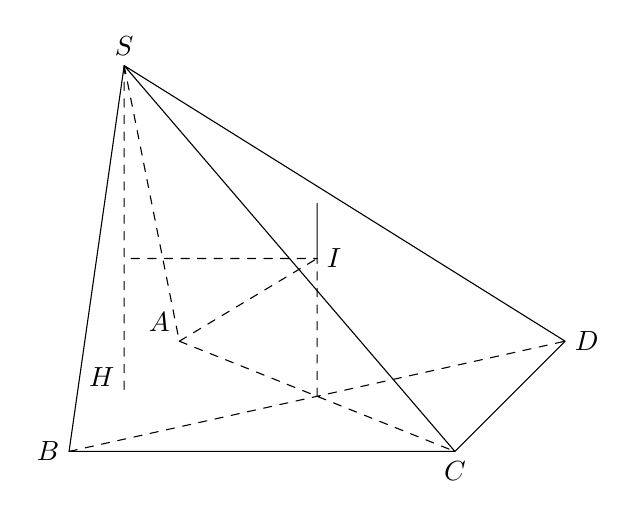
\begin{tikzpicture}[>=stealth, line join=round, line cap=round,scale=0.7]
				\coordinate(A) at(0,0);
				\coordinate(B) at(-2,-2);
				\coordinate(C) at(5,-2);
				\coordinate(D) at(7,0);
				\coordinate(H) at(-1,-1);
				\coordinate(S) at(-1,5);
				\coordinate(I) at(2.5,-1);
				\coordinate(O) at(2.5,1.5);
				\coordinate(P) at(2.5,2.5);
				\coordinate(L) at(-1,1.5);
				\draw[dashed] (S)--(H)(S)--(A)(A)--(C)(B)--(D)(I)--(O)--(L)(A)--(O);
				\draw(B)--(C)--(D)(S)--(C)(S)--(B)(S)--(D)(O)--(P);
				\draw(A) node[above left]{$A$}(B)node[left]{$B$}(C)node[below]{$C$}(D)node[right]{$D$}(S)node[above]{$S$}
				(H)node[above left]{$H$}(O)node[right]{$I$};
				\tkzDrawSegments[dashed](A,B A,D);
				\tkzLabelSegment[above](A,D){2};
				\tkzLabelSegment(A,H){3};
				\tkzDrawPoints(S,A,B,C,D,H,I,O,P,L);
		\end{tikzpicture}}
	}
\end{ex}

%%==========Câu 21
\begin{ex}%[2D1Y5-1]
	\immini
	{Hàm số nào dưới đây có đồ thị dạng như đường cong trong hình bên? 
	\choice
		{$y=-x^{4}+2x^{2}-2$}
		{$y=x^{4}+2x^{2}+2$}
		{\True $y=x^{4}-2x^{2}-1$}
		{$y=-x^{4}+2x^{2}+1$}}
	{\begin{tikzpicture}[scale=1,>=stealth, font=\footnotesize, line join=round, line cap=round]
			\def\a{1} \def\b{-2} \def\c{-1} % Hệ số
			\def\xmin{-2.5} \def\xmax{2.5}
			\def\ymin{-3} \def\ymax{1}
			\draw[->](\xmin,0)--(\xmax,0) node [below]{$x$};
			\draw[->](0,\ymin)--(0,\ymax) node [left]{$y$};
			\node at(0,0) [below left]{$O$};
			\clip(\xmin+0.1,\ymin+0.1) rectangle(\xmax-0.5,\ymax-0.1);
			\draw[smooth,samples=300] plot(\x,{\a*(\x)^4+\b*(\x)^2+\c});
	\end{tikzpicture}}
	\loigiai{
		Từ đồ thị suy ra hệ số $a>0$.\\
		Giao điểm của đồ thị với trục $Oy$ có tung độ âm.\\
		Vậy chỉ có $y=x^{4}-2x^{2}-1$ thoả mãn.
	}
\end{ex}

%%==========Câu 22
\begin{ex}%[1D2B5-5]
	Trong mặt phẳng cho một tập hợp $P$ gồm $7$ điểm, trong đó không có $3$ điểm nào thẳng hàng. Có bao nhiêu tam giác có $3$ đỉnh đều thuộc $P$?
	\choice
	{\True $\mathrm{C}_{7}^{3}$}
	{$36$}
	{$\mathrm{A}_{7}^{3}$}
	{$6$}
	\loigiai{
		Với mỗi tập con gồm $3$ điểm bất kì của $P$, ta tạo được một tam giác với các đỉnh là $3$ điểm đó. Ngược lại, mỗi tam giác có $3$ đỉnh thuộc $P$ tương ứng với một tập con gồm $3$ điểm của $P$.\\
		Vậy số tam giác có $3$ đỉnh thuộc $P$ chính là số các tổ hợp chập $3$ của tập $P$, tức là bằng $\mathrm{C}_{7}^{3}$.
	}
\end{ex}
%%==========Câu 23
\begin{ex}%[2D2B3-2]
	Cho $\log _{2} a=x$ và $\log _{2} b=y\left(a>0, b>0, a^{2} \neq b^{2}\right)$. Tìm biểu diễn của $\log _{a^{-2} b^{3}}\left(a^{4} b\right)$ theo $x$ và $y$.
	\choice
	{\True $\dfrac{4x+y}{3y-2x}$}
	{$\dfrac{4x+y}{3y+2x}$}
	{$\dfrac{x-4y}{3y+2x}$}
	{$\dfrac{4x+y}{-2y+3x}$}
	\loigiai{
		Ta có $\log _{a^{-2} b^{3}}\left(a^{4} b\right)=\dfrac{\log _{2}\left(a^{4} b\right)}{\log _{2}\left(a^{-2} b^{3}\right)}=\dfrac{4 \log _{2} a+\log _{2} b}{-2 \log _{2}a+3 \log _{2}b}=\dfrac{4x+y}{3y-2x}$.
	}
\end{ex}

%%==========Câu 24
\begin{ex}%[2D2B5-2]
	Tập nghiệm của bất phương trình $\left(\dfrac{3}{4}\right)^{2x-4}>\left(\dfrac{3}{4}\right)^{x+1}$ là
	\choice
	{$S=(-1; 2)$}
	{$S=(-\infty;-1)$}
	{$S=[5;+\infty)$}
	{\True $S=(-\infty; 5)$}
	\loigiai{
		Ta có $\left(\dfrac{3}{4}\right)^{2x-4}>\left(\dfrac{3}{4}\right)^{x+1}\Leftrightarrow 2x-4<x+1\Leftrightarrow x<5$.\\
		Vậy tập nghiệm của bất phương trình là $S=(-\infty; 5)$.
	}
\end{ex}

%%==========Câu 25
\begin{ex}%[2D3K3-5]
	Một ô tô đang chạy với vận tốc $15$ (m/s) thì tăng tốc chuyển động nhanh dần với gia tốc $a=3t-8$ (m/s$^{2}$), trong đó $t$ là khoảng thời gian tính bằng giây kể từ lúc tăng vận tốc. Hỏi sau $10$ giây tăng vận tốc, ô tô đi được bao nhiêu mét?
	\choice
	{$150$}
	{\True $250$}
	{$180$}
	{$246$}
	\loigiai{
		Ta có $v(t)=\displaystyle\int(3t-8) \mathrm{\,d} t=\dfrac{3}{2} t^{2}-8t+C$.\\
		Ta có $v(0)=15 \Rightarrow C=15 \Rightarrow v(t)=\dfrac{3}{2} t^{2}-8t+15$.\\
		Sau $10$ giây tăng vận tốc, ô tô đi được số mét là $\displaystyle\int_{0}^{10}\left(\dfrac{3}{2} t^{2}-8t+15\right) \mathrm{\,d} t=\left.\left(\dfrac{1}{2} t^{3}-4 t^{2}+15 t\right)\right|_{0}^{10}=250$.
	}
\end{ex}

%%==========Câu 26
\begin{ex}%[2H3B1-1]
	Trong KG $Oxyz$, cho tam giác $ABC$ có $\overrightarrow{AB}=(-3; 0; 4)$, $\overrightarrow{AC}=(5;-2; 4)$. Độ dài đường trung tuyến $AM$ là
	\choice
	{$2\sqrt{3}$}
	{$5\sqrt{2}$}
	{\True $3\sqrt{2}$}
	{$4\sqrt{2}$}
	\loigiai{
		Ta có $\overrightarrow{AM}=\dfrac{1}{2}(\overrightarrow{AB}+\overrightarrow{AC})=(1;-1; 4) \Rightarrow AM=\sqrt{1^{2}+(-1)^{2}+4^{2}}=3\sqrt{2}$.
	}
\end{ex}
%%==========Câu 27
\begin{ex}%[2D3K2-2]
	Cho hàm số $y=f(x)$ có đạo hàm $f'(x)$ liên tục trên đoạn $[0; 1]$ thoả mãn $f(1)=1$ và $\displaystyle\int_{0}^{1} f(x)\mathrm{\,d}x=2$. Tích phân $\displaystyle\int_{0}^{1} f'(\sqrt{x})\mathrm{\,d}x$ bằng
	\choice
	{$1$}
	{$2$}
	{$-1$}
	{\True $-2$}
	\loigiai{
		Xét tích phân $I=\displaystyle\int_{0}^{1} f'(\sqrt{x})\mathrm{\,d}x$.\\
		Đặt $t=\sqrt{x} \Rightarrow t^{2}=x \Rightarrow 2t \mathrm{\,d} t=\mathrm{\,d} x$.\\
		Đổi cận $x=0 \Rightarrow t=0; x=1 \Rightarrow t=1$.\\
		Vậy $I=\displaystyle\int_{0}^{1} 2t\cdot f'(t) \mathrm{\,d}t=\displaystyle\int_{0}^{1} 2t\mathrm{\,d}\left(f(t)\right)=2t\cdot f(t)\bigg|_{0}^{1}-\displaystyle\int_{0}^{1} 2f(t) \mathrm{\,d}t=2f(1)-2\displaystyle\int_{0}^{1} f(t)\mathrm{\,d}t=2\cdot1-2\cdot2=-2$.
	}
\end{ex}

%%==========Câu 28
\begin{ex}%[2D4Y1-2]
	Tìm tọa độ điểm biểu diễn của số phức $z=\dfrac{(2-3i)(4-i)}{3+2i}$.
	\choice
	{$(-1; 4)$}
	{$(1; 4)$}
	{$(1;-4)$}
	{\True $(-1;- 4)$}
	\loigiai{
		Ta có $z=\dfrac{(2-3i)(4-i)}{3+2i}=-1-4i$ nên điểm biểu diễn số phức $z=-1-4i$ có tọa độ $(-1;-4)$.
	}
\end{ex}

%%==========Câu 29
\begin{ex}%[2D3K2-2]
	Cho hàm số $f(x)$ liên tục trên $\mathbb{R}$ thỏa mãn $\displaystyle\int_{0}^{2021} f(x)\mathrm{\,d}x=2$.\\
	Khi đó tích phân $\displaystyle\int_{0}^{\sqrt{e^{2021}}-1}\dfrac{x}{x^{2}+1} f\left(\ln \left(x^{2}+1\right)\right)\mathrm{\,d}x$ bằng
	\choice
	{$2$}
	{$3$}
	{$4$}
	{\True $1$}
	\loigiai{
		Đặt $u=\ln \left(x^{2}+1\right) \Rightarrow \mathrm{\,d} u=\dfrac{2x}{x^{2}+1}\mathrm{\,d}x$.\\
		Đổi cận $\heva{&x=0  \Rightarrow u=0\\&x=\sqrt{e^{2021}-1}  \Rightarrow u=2021}$.\\
		Khi đó $\displaystyle\int_{0}^{\sqrt{e^{2021}-1}}\dfrac{x}{x^{2}+1} f\left(\ln \left(x^{2}+1\right)\right)\mathrm{\,d}x=\dfrac{1}{2} \displaystyle\int_{0}^{2021} f(u)\mathrm{\,d}u=1$.
	}
\end{ex}

%%==========Câu 30
\begin{ex}%[2H3K2-4]
	Trong KG $Oxyz$, cho điểm $E(1; 1;-1)$. Gọi $A$, $B$ và $C$ lần lượt là hình chiếu của $E$ trên các trục tọa độ $Ox$, $Oy$, $Oz$. Điểm nào sau đây thuộc mặt phẳng $(ABC)$?
	\choice
	{$N(0; 1; 1)$}
	{\True $Q(1; 1; 1)$}
	{$M(2; 1;-1)$}
	{$P(1;-1; 1)$}
	\loigiai{
		Phương trình mặt phẳng $(ABC)\colon\dfrac{x}{1}+\dfrac{y}{1}-\dfrac{z}{1}=1$. Nên thử vào ta được $Q(1; 1; 1) \in(ABC)$.
	}
\end{ex}

%=====================

 %%==========Câu 31
\begin{ex}%[2D2B4-1]
	Tìm tập xác định của hàm số $y=\ln (2-x)+{x}^{\pi}$
	\choice 
	{$(0;+\infty)$}
	{$(-\infty;2)$}
	{$(-\infty;2]$}
	{\True $(0;2)$}
	\loigiai{
		Điều kiện: $\heva{&2-x>0\\&x>0} \Leftrightarrow 0<x<2$.\\
		Tập xác định của hàm số là $\mathscr{D}=(0;2)$.
	} 
\end{ex} 

%%==========Câu 32
\begin{ex}%[2D1B3-1] 
	Tìm giá trị nhỏ nhất của hàm số $y=x^3-3x^2-9x+5$ trên đoạn $[-2;2]$.
	\choice 
	{$3$}
	{\True $-17$}
	{$-1$}
	{$-22$}
	\loigiai{
		Ta có $y'=3x^2-6x-9$, cho $y'=0 \Leftrightarrow 3x^2-6x-9=0 \Leftrightarrow \hoac{&x=-1\\&x=3&(\text{loại}).}$\\
		Ta có $\heva{&y(-2)=3\\&y(-1)=10\\&y(2)=-17} \Rightarrow \min\limits_{[-2;2]}y=-17$.} 
\end{ex} 

%%==========Câu 33
\begin{ex}%[2D3B2-1] 
	Cho $\displaystyle\int\limits_{1}^5 f(x)\mathrm{\,d}x=5$ và $\displaystyle\int\limits_{1}^2 f(x)\mathrm{\,d}x=7$, $f(x)$ liên tục trên đoạn $[1;5]$. Tính $\displaystyle\int\limits_{2}^5 f(x)\mathrm{\,d}x$.
	\choice 
	{$-12$}
	{$-2$}
	{\True $2$}
	{$12$}
	\loigiai{
		Ta có $$\displaystyle\int\limits_{1}^2 f(x)\mathrm{\,d}x+\displaystyle\int\limits_{2}^5 f(x)\mathrm{\,d}x=\displaystyle\int\limits_{1}^5 f(x)\mathrm{\,d}x\Rightarrow \displaystyle\int\limits_{2}^5 f(x)\mathrm{\,d}x=\displaystyle\int\limits_{1}^5 f(x)\mathrm{\,d}x-\displaystyle\int\limits_{1}^2 f(x)\mathrm{\,d}x=5-7=-2.$$} 
\end{ex} 

%%==========Câu 34
\begin{ex}%[2H3B1-3] 
	Trong KG $Oxyz$, cho hai điểm $I(1;0;-1)$ và $A(2;2;-3)$. Mặt cầu $(S)$ tâm $I$ và đi qua điểm $A$ có phương trình là
	\choice 
	{$(x-1)^2+y^2+(z+1)^2=3$}
	{\True $(x-1)^2+y^2+(z+1)^2=9$} 
	{$(x+1)^2+y^2+(z-1)^2=9$}
	{$(x+1)^2+y^2+(z-1)^2=3$}
	\loigiai{
		Ta có bán kính mặt cầu $R=IA=3$.\\
		Vậy phương trình mặt cầu $(S)\colon (x-1)^2+y^2+(z+1)^2=9$.} 
\end{ex}

%%==========Câu 35
\begin{ex}%[2H1Y3-2]
	Cho hình chóp $S.ABCD$ có đáy $ABCD$ là hình chữ nhật, $AB=2a,\,BC=a,\,SA=a\sqrt{3}$ và $SA$ vuông góc với mặt đáy $(ABCD)$. Thể tích $V$ của khối chóp $S.ABCD$ bằng
	\choice 
	{\True $V=\dfrac{2a^3\sqrt{3}}{3}$}
	{$V=2a^3\sqrt{3}$}
	{$V=a^3\sqrt{3}$}
	{$V=\dfrac{a^3\sqrt{3}}{3}$}
	\loigiai{
		Ta có $${V_{S.ABCD}}=\dfrac{1}{3}AB\cdot BC\cdot SA=\dfrac{1}{3}\cdot 2a\cdot a\cdot a\sqrt{3}=\dfrac{2{{a}^3}\sqrt{3}}{3}.$$}
\end{ex} 

%%==========Câu 36
\begin{ex}%[2H3B2-3] 
	Trong KG $Oxyz$, mặt phẳng $(P)$ đi qua điểm $M(-2; 1; 3)$ và chứa trục hoành có phương trình là
	\choice 
	{\True $(P)\colon 3y-z=0$}
	{$(P)\colon x-y+z=0$}
	{$(P)\colon y+z-4=0$}
	{$(P)\colon 3y+z-6=0$}
	\loigiai{
		Ta có $\overrightarrow{OM}=(-2;1;3)$.Trục hoành có véc-tơ chỉ phương là $\overrightarrow{i}=(1;0;0)$.\\
		Suy ra $\vec{n}=[\overrightarrow{OM},\overrightarrow{i}]=(0;3;-1)$.\\
		Khi đó phương trình mặt phẳng $(P)\colon 3y-z=0$
	}
\end{ex} 

%%==========Câu 37
\begin{ex}%[2H1B3-3] 
	Cho hình hộp $ABCD.A'B'C'D'$. Tính tỷ số thể tích của khối tứ diện $BDA'C'$ và khối hộp $ABCD.A'B'C'D'$.
	\choice 
	{${\dfrac{1}{5}}$}
	{${\dfrac{2}{5}}$}
	{\True ${\dfrac{1}{3}}$}
	{${\dfrac{2}{3}}$}
	\loigiai{
		\immini
		{Ta có $V_{ABCD.A'B'C'D'}=V_{BDA'C'}+V_{ABDA'}+V_{BCDC'}+V_{A'B'C'B}+V_{A'C'D'D}$.\\
		Mà $V_{ABDA'}=V_{BCDC'}=V_{A'B'C'B}=V_{A'C'D'D}$.\\
		Và $V_{ABDA'}=\dfrac{1}{3}\cdot \mathrm{d}\left(A',(ABD)\right)\cdot S_{ABD}=\dfrac{1}{3}\cdot \mathrm{d}\left(A',(ABCD)\right)\cdot\dfrac{S_{ABCD}}{2}=\dfrac{V_{ABCD.A'B'C'D'}}{6}$.\\
		$$\begin{array}{lll}
		V_{BDA'C'}&=V_{ABCD.A'B'C'D'}-(V_{ABDA'}+V_{BCDC'}+V_{A'B'C'B}+V_{A'C'D'D})\\
		&=V_{ABCD.A'B'C'D'}-4\cdot V_{ABDA'}\\
		&=V_{ABCD.A'B'C'D'}-4\cdot\dfrac{1}{6}\cdot V_{ABCD.A'B'C'D'}=\dfrac{V_{ABCD.A'B'C'D'}}{3}.
		\end{array}$$
		Suy ra $\dfrac{V_{BDA'C'}}{V_{ABCD.A'B'C'D'}}=\dfrac{1}{3}$.}
		{\begin{tikzpicture}[smooth,line join=round, line cap=round, font=\scriptsize,scale=0.5]
			\path 
			(0,0) coordinate(D)
			(-140:3.5) coordinate(A)
			(0:6) coordinate(C)
			($(A)+(C)-(D)$) coordinate(B)
			(75:5) coordinate(D')
			($(D')+(A)-(D)$) coordinate(A')
			($(D')+(C)-(D)$) coordinate(C')
			($(D')+(B)-(D)$) coordinate(B');
			\draw[densely dashed](A)--(D)--(C)(D)--(D')(A')--(D)--(C')(D)--(B);
			\draw(A)--(A')--(D')--(C')--(B')--(B)--(C)--(C')(A')--(B')(A)--(B)--(C')--(A')--(B);
			\foreach \x/\g in {A/-135,B/-90,C/0,D/-90,A'/180,D'/150,C'/45,B'/-30}
			\fill(\x) circle(1.5pt)+(\g:3mm) node {$\x$};
		\end{tikzpicture}}
	}
\end{ex}

%%==========Câu 38
\begin{ex}%[2H3Y1-1]
	Trong KG $Oxyz$, cho điểm $M(3; 2;-1)$. Hình chiếu vuông góc của điểm $M$ lên trục $Oz$ là điểm
	\choice 
	{\True $M_1(0;0;-1)$}
	{$M_2(3;2;0)$}
	{$M_4(0;2;0)$}
	{$M_3(3;0;0)$}
	\loigiai{
		Hình chiếu vuông góc của điểm $M(3; 2;-1)$ lên trục $Oz$ là điểm $M_1(0;0;-1)$.}
\end{ex} 

%%==========Câu 39
\begin{ex}%[2D3K2-4] 
	Biết $\displaystyle\int\limits_0^{\tfrac{\pi}{2}}\dfrac{(m^2+1)\cos x-2m\sin x}{\cos x+\sin x}\mathrm{\,d}x=\pi$ ($m$ là tham số thực). Tích các giá trị của $m$ là
	\choice 
	{$-1$}
	{$-4$}
	{\True $-3$}
	{$-2$}
	\loigiai{
		Xét $I=\displaystyle\int\limits_0^{\tfrac{\pi}{2}}\dfrac{(m^2+1)\cos x-2m\sin x}{\cos x+\sin x}\mathrm{\,d}x$. \qquad $(1)$\\
		Ta sử dụng tính chất $\displaystyle\int\limits_a^b f(x)\mathrm{\,d}x=\displaystyle\int\limits_{a}^b f(b+a-x)\mathrm{\,d}x$. Khi đó
		$$I=\displaystyle\int\limits_0^{\tfrac{\pi}{2}}{\dfrac{(m^2+1)\cos\left(\dfrac{\pi}{2}-x\right)-2m\sin\left(\dfrac{\pi}{2}-x\right)}{\cos\left(\dfrac{\pi}{2}-x\right)+\sin\left(\dfrac{\pi}{2}-x\right)}}\mathrm{\,d}x=\displaystyle\int\limits_0^{\tfrac{\pi}{2}}{\dfrac{(m^2+1)\sin x-2m\cos x}{\sin x+\cos x}}\mathrm{\,d}x. \qquad (2)$$
		Lấy $(1)+(2)$, ta có
		$$\begin{array}{lll}
		&2I=\displaystyle\int\limits_{0}^{\tfrac{\pi}{2}}\dfrac{(m^2+1)(\sin x+\cos x)-2m(\sin x+\cos x)}{\cos x+\sin x}\mathrm{\,d}x\\
		\Leftrightarrow &2I= \displaystyle\int\limits_{0}^{\tfrac{\pi}{2}}(m^2-2m+1)\mathrm{\,d}x\\
		\Leftrightarrow &2I=(m-1)^2\cdot\dfrac{\pi}{2}\\
		\Leftrightarrow &2\pi=(m-1)^2\cdot\dfrac{\pi}{2}\\
		\Leftrightarrow &(m-1)^2=4 \Leftrightarrow \hoac{&m-1=2\\&m-1=-2} \Leftrightarrow \hoac{&m=3\\&m=-1.}
		\end{array}$$
		Suy ra tích các giá trị của tham số $m$ là $-3$.
	}
\end{ex}

%%==========Câu 40
\begin{ex}%[2H3B2-8]
	Trong KG $Oxyz$, cho ba điểm $A(a;0;0),\,B(0;b;0),\,C(0;0;c)$, trong đó $a>0,\,b>0,\,c>0$. Mặt phẳng $(ABC)$ đi qua điểm $I(1;2;3)$ sao cho thể tích khối tứ diện $OABC$ đạt giá trị nhỏ nhất. Khi đó các số $a,\,b,\,c$ thoả mãn đẳng thức nào dưới đây?
	\choice 
	{$a+b+c=12$}
	{\True $a+b+c=18$}
	{$a^2+b=c-6$}
	{$a+b-c=6$}
	\loigiai{
		Mặt phẳng $(ABC)\colon \dfrac{x}{a}+\dfrac{y}{b}+\dfrac{z}{c}=1$.\\
		Điểm $I(1;2;3)\in(ABC) \Rightarrow \dfrac{1}{a}+\dfrac{2}{b}+\dfrac{3}{c}=1$.\\
		Ta có $1=\dfrac{1}{a}+\dfrac{2}{b}+\dfrac{3}{c}\ge 3\sqrt[3]{\dfrac{6}{abc}} \Leftrightarrow abc\ge 162$.\\
		Khi đó $V_{OABC}=\dfrac{abc}{6}\ge\dfrac{162}{6}=27$.\\
		Dấu \lq\lq =\rq\rq\, xảy ra $\heva{&\dfrac{1}{a}=\dfrac{2}{b}=\dfrac{3}{c}=\dfrac{1}{3}\\&1=\dfrac{1}{a}+\dfrac{2}{b}+\dfrac{3}{c}} \Rightarrow \heva{&a=3\\&b=6\\&c=9} \Rightarrow a+b+c=18$.
		}
\end{ex} 

%%==========Câu 41
\begin{ex}%[2D1K3-1]
	\immini
	{Cho hàm số $y=f(x)$ liên tục trên $\mathbb{R}$ và có đồ thị là hình vẽ. Gọi $M$, $m$ theo thứ tự là giá trị lớn nhất và giá trị nhỏ nhất của hàm số $y=|f(x)-2|^3-3\left(f(x)-2\right)^2+5$ trên đoạn $[-1;3]$. Tính $M\cdot m$.
	\choice 
		{\True $55$}
		{$2$}
		{$54$}
		{$3$}}
	{\begin{tikzpicture}[smooth,line join=round, line cap=round, font=\scriptsize,scale=0.6,>=latex,yscale=0.8]
		\draw[->](-2,0)--(4,0) node[below] {$x$};
		\draw[->](0,-2)--(0,8) node[right] {$y$};
		\draw[densely dashed](-1,0) node[below] {$-1$}|-(0,3) node[right] {$3$}(1,0) node[below] {$1$} |-(0,1) node[left] {$1$}(3,0) node[below] {$3$} |-(0,7) node[left] {$7$}; 
		\draw(-1.5,7.5)..controls+(-90:0.1) and+(-180:0.1)..(-1,3)..controls+(0:0.1) and+(180:0.2)..(-0.5,3.6)..controls+(0:0.4) and+(90:0.2)..(1,1)..controls+(90:0.1)..(3,7) ;	
	\end{tikzpicture}}
	\loigiai{
		Đặt $t=|f(x)-2|$. Ta có
		$$1\le f(x)\le 7,\, \forall x\in [-1;3] \Rightarrow 0\le |f(x)-2|\le 5, \,\forall x \in [-1;3].$$
		Xét hàm số $f(t)=t^3-3t^2+5$ với $t\in [0;5]$.\\
		Ta có $f'(t)=3t^2-6t$, cho $f'(t)=0 \Leftrightarrow \hoac{&t=0\\&t=2.}$\\
		Khi đó $\heva{&f(5)=55\\&f(2)=1\\&f(0)=5} \Rightarrow \heva{&\max\limits_{t\in [0;5]} f(t)=f(5)=55\\&\min\limits_{t\in [0;5]} f(t)=f(2)=1.}$
	}
\end{ex} 

%%==========Câu 42
\begin{ex}%[2D2B4-2]
	Biết $F(x)=(ax^2+bx+c)e^{-x}$ là một nguyên hàm của hàm số $f(x)=(2x^2-5x+2)e^{-x}$ trên $\mathbb{R}$. Tính giá trị của biểu thức $f[F(0)]$.
	\choice 
	{$20{e^2}$}
	{\True $9e$}
	{$-{e^{-1}}$}
	{$3e$} 
	\loigiai{
		Ta có $f(x)=F'(x)$. Suy ra 
		$$\begin{array}{lll}
		&(2x^2-5x+2)e^{-x} &=\left[(ax^2+bx+c)e^{-x}\right]'\\
		\Rightarrow &(2x^2-5x+2)e^{-x} &=(2ax+b)e^{-x}-(ax^2+bx+c)e^{-x}\\
		\Rightarrow &(2x^2-5x+2)e^{-x} &=(-ax^2+(2a-b)x+b-c)e^{-x}.
		\end{array}$$
		Suy ra $\heva{&-a=2\\&2a-b=-5\\&b-c=2} \Leftrightarrow \heva{&a=-2\\&b=1\\&c=-1.}$\\
		Khi đó $F(x)=(-2x^2+x-1)e^{-x} \Rightarrow F(0)=-1 \Rightarrow f[F(0)]=9e$.
	}
\end{ex}


%%==========Câu 43
\begin{ex}%[2H1K3-3]
	Cho hình chóp $S.ABCD$ có đáy là hình bình hành, có thể tích bằng $24$ cm$^3$. Gọi $E$ là trung điểm của $SC$. Một mặt phẳng chứa $AE$ cắt các cạnh $SB$ và $SD$ lần lượt tại $M$ và $N$. Tìm giá trị nhỏ nhất của thể tích $S.AMNE$.
	\choice
	{$7$ cm$^3$}
	{$6$ cm$^3$}
	{\True $8$ cm$^3$}
	{$9$ cm$^3$}
	\loigiai{
		\immini
		{Đặt $\dfrac{SB}{SM}=x$, $\dfrac{SD}{SN}=y$, khi đó ta có\\
		$\heva{&x+y=3\\&\dfrac{V_{S.AMEN}}{V_{S.ABCD}}=\dfrac{1+2+x+y}{4\cdot 1\cdot 2\cdot x\cdot y}} \Leftrightarrow \heva{&y=3-x\\&V_{S.AMEN}=\dfrac{3+x+y}{8xy}\cdot24}$\\
		$\Leftrightarrow \heva{&y=3-x\\&V_{S.AMEN}=\dfrac{18}{x(3-x)}.}$\\
		Đặt $f(x)=\dfrac{18}{x(3-x)} \Rightarrow f'(x)=\dfrac{36x-54}{(3x-x^2)^2}$.\\
		Ta có $\min f(x)=f\left(\dfrac{3}{2}\right)=8$.\\
		Vậy thể tích nhỏ nhất của khối chóp $S.AMEN$ bằng $8$ cm$^3$.}
		{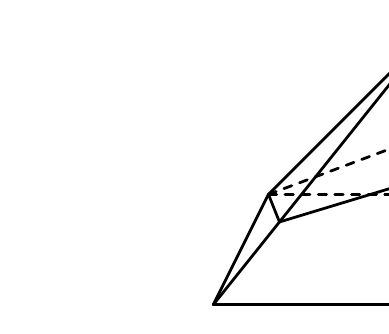
\begin{tikzpicture}[smooth,line join=round, line cap=round, font=\scriptsize,scale=0.7]	
			\path
			(2,3) coordinate(A)
			(1,1) coordinate(B)
			(6,1) coordinate(C)
			(7,3) coordinate(D)
			(5,6) coordinate(S)
			(5.5,3.5) coordinate(E)
			(6,4.5) coordinate(N)
			(2.2,2.5) coordinate(M);
			\tkzLabelPoint[left](A){$A$}
			\tkzLabelPoint[below](B){$B$}
			\tkzLabelPoint[below](C){$C$}
			\tkzLabelPoint[below right](D){$D$}
			\tkzLabelPoint[above](S){$S$}
			\tkzLabelPoint[right](E){$E$}
			\tkzLabelPoint[right](N){$N$}
			\tkzLabelPoint[below right](M){$M$}
			\tkzDrawPoints[fill=red](A,B,C,D,S,E,N,M)
			\draw[ line width=1](A)--(B);
			\draw[ line width=1](A)--(S);
			\draw[ line width=1 , dashed](A)--(D);
			\draw[ line width=1](S)--(B);
			\draw[ line width=1](C)--(B);
			\draw[ line width=1](C)--(D);
			\draw[ line width=1](C)--(S);
			\draw[ line width=1](D)--(S);
			\draw[ line width=1](E)--(N);
			\draw[ line width=1, dashed](A)--(N);
			\draw[ line width=1](E)--(M);
			\draw[ line width=1](A)--(M);
		\end{tikzpicture}}
	}
\end{ex}

%%==========Câu 44
\begin{ex}%[2D2K4-4]
	Cho $x$, $y$ là các số thực và $x$ dương thỏa mãn $\log_{2}\dfrac{1-y^2}{x}=3(x+y^2-1)$. Biết giá trị lớn nhất của biểu thức $P=\dfrac{1-y^2+\sqrt{9x^2+1}}{8x^2+y^2+x}$ bằng $\dfrac{a\sqrt{b}}{c^2}$ với $a$, $b$, $c$ là các số nguyên tố. Tính giá trị của biểu thức $T=a+b+c$.
	\choice
	{\True $T=7$}
	{$T=10$}
	{$T=12$}
	{$T=8$}
	\loigiai{
		Điều kiện $-1<y<1$.\\
		Ta có $\log_{2}\dfrac{1-y^2}{x}=3(x+y^2-1) \Leftrightarrow \log_{2}(1-y^2)+3(1-y^2)=\log_{2}x+3x$.\\
		Xét $f(t)=\log_{2}t+3t$ với $t>0$ suy ra $f'(t)=\dfrac{1}{t\ln 2}+3$.\\
		Khi đó hàm đã cho đồng biến trên tập xác định.\\
		Suy ra $1-y^2=x$.\\
		Ta có $P=\dfrac{1-y^2+\sqrt{9x^2+1}}{8x^2+1}=\dfrac{1}{\sqrt{9x^2+1}}-x$.\\
		Khảo sát hàm số $f(x)=\dfrac{1}{\sqrt{9x^2+1}}-x$ ta được $\max f(x)=f\left(\dfrac{1}{\sqrt{72}}\right)=\dfrac{3\sqrt{2}}{4}$.\\
		Suy ra $T=a+b+c=7$.
	}
\end{ex}

%%==========Câu 45
\begin{ex}%[2D4K5-1]
	Cho $\left|z-1-i\right|=2$. Giá trị lớn nhất của $P=\sqrt{3}\left|z-3+3i\right|+\left|z+2-7i\right|$ là
	\choice
	{$\sqrt{340}$}
	{$\sqrt{170}$}
	{$\sqrt{\dfrac{425}{3}}$}
	{\True $\sqrt{255}$}
	\loigiai{
		Gọi số phức $z=x+yi$, $(x; y \in \mathbb{R})$.\\
		Theo đề bài $\left|z-1-i\right|=2 \Leftrightarrow \left|x-1+(y-1)i\right|=2 \Leftrightarrow x^2+y^2-2x-2y=2$.\\
		Ta có 
		\allowdisplaybreaks
		$\begin{aligned}[t]
		P&=\sqrt{3}\left|z-3+3i\right|+\left|z+2-7i\right|\\
		&=\sqrt{(x-3)^2+(y+3)^2}+\sqrt{(x+2)^2+(y-7)^2}\\
		&=\sqrt{3[(x-3)^2+(y+3)^2]}+\dfrac{1}{\sqrt{2}}\sqrt{2\left[(x+2)^2+(y-7)^2\right]}.
		\end{aligned}$\\
		Áp dụng bất đẳng thức Cauchy-Schwars, ta có\\
		$P\leq\sqrt{1^2+(\dfrac{1}{\sqrt{2}})^2}\cdot\sqrt{3[(x-3)^2+(y+3)^2]+2[(x+2)^2+(y-7)^2]}$.\\
		Hay $P \leq\sqrt{\dfrac{3}{2}}\sqrt{5(x^2+y^2-2x-2y+32)}=\sqrt{\dfrac{3}{2}}\sqrt{5(2+32)}=\sqrt{255}$.\\
		Đẳng thức xảy ra khi $\heva{&\dfrac{\sqrt{3[(x-3)^2+(y+3)^2]}}{1}=\dfrac{\sqrt{2[(x+2)^2+(y-7)^2]}}{\dfrac{1}{\sqrt{2}}}\\&x^2+y^2-2x-2y=2}$\\
		$\Leftrightarrow \heva{&3\left[(x-3)^2+(y+3)^2\right]=4\left[(x+2)^2+(y-7)^2\right]\\&x^2+y^2-2x-2y=2} \Leftrightarrow \heva{&x^2+y^2+34x-74y+158=0\\&x^2+y^2-2x-2y=2}$\\
		$\Leftrightarrow \heva{&36x-72y+160=0\\&x^2+y^2-2x-2y=2} \Leftrightarrow \heva{&9x-8y+40=0\\&x^2+y^2-2x-2y=2}$\\
		$\Leftrightarrow \heva{&x=2y-\dfrac{40}{9}\\&(2y-\dfrac{40}{9})^2+y^2-2(2y-\dfrac{40}{9})-2y-2=0} \Leftrightarrow \heva{&x=2y-\dfrac{40}{9}\\&5y^2-\dfrac{214}{9}y-\dfrac{2158}{81}=0. \quad (*)}$\\
		Phương trình $(*)$ có $\Delta'=\left(\dfrac{107}{9}\right)^2-5\cdot\dfrac{2158}{81}=\dfrac{659}{81}>0$ nên hệ trên có nghiệm.\\
		Vậy giá trị lớn nhất của $P$ là $\sqrt{255}$.
	}
\end{ex}

%%==========Câu 46
\begin{ex}%[2D2K5-5]
	Có bao nhiêu số nguyên $a, (a\geq 2)$ sao cho tồn tại số thực $x$ thỏa mãn \linebreak $\ln \left(a^{\log x^4}+4a^{\log x^2}+4\right)=\dfrac{\ln (x-2)}{\log a}$?
	\choice
	{\True $2$}
	{$3$}
	{$1$}
	{$9$}
	\loigiai{
		Ta có $\ln (a^{\log x^4}+4a^{\log x^2}+4)=\dfrac{\ln (x-2)}{\log a} \Leftrightarrow \ln (a^{4\log x}+4a^{2\log x}+4))=\dfrac{\ln (x-2)}{\log a}$. \quad $(1)$\\
		Đặt $a^{2\log x}+2=t \Rightarrow \log a \cdot 2\log x=\log(t-2) \Rightarrow \log a=\dfrac{\log(t-2)}{2\log x}$.\\
		Khi đó, $(1)$ trở thành $\ln t \cdot\ln (t-2)=\ln x\cdot \ln (x-2)$. \quad  $(2)$\\
		Xét hàm $f(u)=\ln u \cdot \ln (u-2)$.\\
		Ta có $f'(u)=\dfrac{\ln (u-2)}{u}+\dfrac{\ln u}{u-2}>0, \forall u>2$.\\
		Do đó, $(2)\Leftrightarrow x=a^{2\log x}+2=x\Leftrightarrow x-x^{2\log a}=2$. \quad  $(3)$\\
		Suy ra $x>x^{2\log a}\Leftrightarrow 2\log a<1\Leftrightarrow \log a<\dfrac{1}{2}\Leftrightarrow a <\sqrt{10} \Rightarrow a \in\left\{2;3\right\} $.\\
		Với $a=2$ thì $(3)$ trở thành $x^{2\log 2}-x+2=0$.\\
		Hàm số $g(x)=x^{2\log 2}-x+2$ liên tục trên $[2;10]$ và $g(2)\cdot g(10)=2^{2\log 2}\cdot (-4)<0$ nên phương trình $g(x)=0$ có nghiệm thuộc khoảng $(2;10)$.\\
		Với $a=3$ thì $(3)$ trở thành $x^{2\log 3}-x+2=0$.\\
		Hàm số $g(x)=x^{2\log 3}-x+2$ liên tục trên $[2;100]$ và $g(2)\cdot g(100)=2^{2\log 3}\cdot(-17)<0$ nên phương trình $g(x)=0$ có nghiệm thuộc khoảng $(2;100)$.\\
		Vậy có $2$ giá trị nguyên $a$ thỏa mãn đề bài.
	}
\end{ex}

%%==========Câu 47
\begin{ex}%[Dự án 15-TeamTeXHoa-Chuyên Lam Sơn Thanh Hóa-Hoàng Blue]%[2D1G2-2]
	\immini
	{Cho hàm số $y=f(x)$ xác định trên $\mathbb{R}$ và có đồ thị hàm số $y=f'(x)$ như hình. Số giá trị nguyên của tham số $m\in(-10;10)$ để hàm số $y=f\left(x^2-2\left|x\right|+\dfrac{m}{2}\right)$ có $9$ điểm cực trị là
	\choice
	{\True $11$}
	{$12$}
	{$9$}
	{$10$}}
	{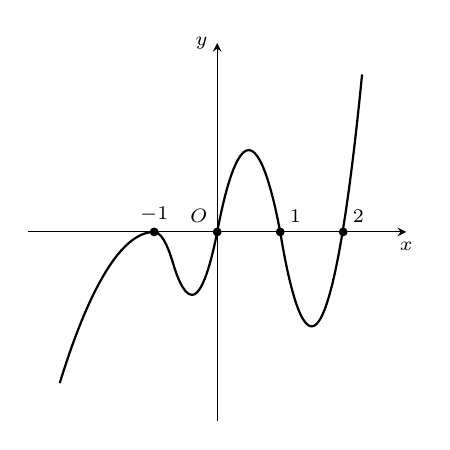
\begin{tikzpicture}[>=stealth,x=1.0cm,y=1.0cm,scale=0.8]
		\draw[color=gray,dash pattern=on 1pt off 1pt,xstep=1.0cm,ystep=1.0cm];
		\draw[->](-3,0)--(3,0) node[below] {\scriptsize $x$};
		\draw[->](0,-3)--(0,3) node[left] {\scriptsize $y$};
		\draw(0,0) node[above left] {\scriptsize $O$} 
		(-1,0) node[above]{\scriptsize $-1$} 
		(1,0) node[above right]{\scriptsize $1$}
		(2,0) node[above right]{\scriptsize $2$};
		\draw[thick,color=black](-2.5,-2.4) parabola bend(-1,0)(-0.7,-0.5)(-0.7,-0.5) parabola bend(-.4,-1)(0,0)(0,0) parabola bend(.5,1.3) (1,0)(1,0) parabola bend(1.5,-1.5)(2.3,2.5);
		%\draw[dashed](-3,0)--(-3,2)--(0,2)(0,-2)--(1,-2)--(1,0)(3,0)--(3,-4)--(0,-4);
		\fill[black](-1,0) circle[radius=2pt](0,0) circle[radius=2pt](1,0) circle[radius=2pt]
		(2,0) circle[radius=2pt];
	\end{tikzpicture}}
	\loigiai{
		Xét hàm số $g(x)=f\left(x^2-2x+\dfrac{m}{2}\right)$ $\Rightarrow g'(x)=\left(2x-2\right)\cdot f'\left(x^2-2x+\dfrac{m}{2}\right)$.\\
		Nhận xét: dựa vào đồ thị ta thấy $f'(x)=0 \Leftrightarrow \hoac{&x=-1\left(\text{bội chẵn}\right)\\&x\in\{0;1;2\}.}$\\
		Cho $g'(x)=0\Leftrightarrow \hoac{&x=1\\&f'\left(x^2-2x+\dfrac{m}{2}\right)=0}\Leftrightarrow \hoac{&x=1\\&x^2-2x+\dfrac{m}{2}=0\\&x^2-2x+\dfrac{m}{2}=1\\&x^2-2x+\dfrac{m}{2}=2}\Leftrightarrow \hoac{&x=1\\&\dfrac{m}{2}=\underbrace{-x^2+2x}_{h_1(x)}\\&\dfrac{m}{2}=\underbrace{-x^2+2x+1}_{h_2(x)}\\&\dfrac{m}{2}=\underbrace{-x^2+2x+2}_{h_3(x)}.}$\\
		Khi đó ta có bảng biến thiên chung của cả $3$ hàm số $h_1(x)$, $h_2(x)$, $h_3(x)$ như sau
		\begin{center}
			\begin{tikzpicture}[scale=1.2]
				%	\draw[thin,opacity=.5](-1,-4) grid 	(9,1);
				\def\f(#1){-4}
				\foreach \i/\x in
				{0/x,1.25/-\infty,4/0,6/1,8.25/+\infty}
				\path(\i,.5) node{$\x$};
				\foreach \i/\x in
				{0/h(x)}
				\path(\i,-2) node{$\x$};
				\draw(-1,1)--(9,1)--(9,-4)--(-1,-4)--(-1,1);
				\draw(-1,0)--(9,0)
				(.75,1)--(.75,-4);
				\draw(6,-.3)node[below]{$3$};
				\draw(6,-1.5)node[below]{$2$};
				\draw(6,-2.3)node[below]{$1$};
				\draw(4.3,-2.2) node[left]{$1$} (4.3,-3) node[left]{$0$};
				\draw [-stealth](4.3,-1.5) node[left]{$2$}--(5.9,-.3);
				\draw [-stealth](6.1,-.3)--(8.25,-3.6)node[right]{$-\infty$};
				\draw [-stealth,red](4.3,-2.2)--(5.9,-1.5);
				\draw [-stealth,red](6.1,-1.5)--(8,-3.6);
				\draw [-stealth,red](4.3,-3)--(5.9,-2.3);
				\draw [-stealth,red](6.1,-2.3)--(7.8,-3.7);
				\fill[pattern=north east lines,smooth](.75,0)--plot[domain=.75:4](\x,{\f(\x)})--(4,0)-- cycle;
				\clip(-1,-5) rectangle(5,-5);
				\draw[smooth,red, line width=1]
				plot[domain=-.5:8.5]
				(\x,{\f(\x)});
			\end{tikzpicture}
		\end{center}
		Yêu cầu bài toán $\Leftrightarrow g(x)$ có $4$ điểm cực trị có hoành độ dương $\Leftrightarrow \hoac{&\dfrac{m}{2}\le 0\\&1<\dfrac{m}{2}<2} \Leftrightarrow \hoac{&m\le 0\\&2<m<4.}$\\
		Do $m\in \mathbb{Z},m\in(-10;10) \Rightarrow m\in\left\{-9;-8;\ldots;0;3\right\}$. Vậy có tất cả $11$ giá trị thỏa mãn.}
\end{ex}
%%==========Câu 48
\begin{ex}%[Dự án 15-TeamTeXHoa-Chuyên Lam Sơn Thanh Hóa-Hoàng Blue]%[1D2K2-3]
	Cho đa giác đều $A_1A_2\ldots A_{20}$. Số ngũ giác có $5$ đỉnh lấy từ $20$ điểm $A_1,A_2,\ldots, A_{20}$ và có đúng $1$ cạnh là cạnh của đa giác $A_1A_2\ldots A_{20}$ là
	\choice
	{$9100$}
	{\True $7280$}
	{$4400$}
	{$5720$}
	\loigiai{
		Ta gọi đặc biệt một cạnh của đa giác là $x$, vì đa giác có $20$ đỉnh nên có $20$ cạnh $x$ như thế.\\
		Ta cần đi tìm số ngũ giác đi qua cạnh $x$ và không kề nhau trong $18$ điểm còn lại của đa giác (trừ hai điểm tạo thành cạnh $x$).\\
		Bài toán trở thành chia $3$ điểm vào một dãy $18$ chỗ trống sao cho không có hai điểm nào kề nhau.\\
		Gọi khoảng cách giữa hai điểm là $y$, từ giả thiết ta có
		$y(1)+y(2)+y(3)+y(4)=15$.
		\begin{itemize}
			\item Theo bài toán chia kẹo Euler: Chọn $4-1=3$ vị trí đặt vách ngăn trong $15-1=14$ vị trí nên cách chọn là $\mathrm{C}_{14}^3$. 
			\item Số cạnh $x$ là $20$ cạnh .
		\end{itemize}
		Vậy số cách chọn là $20\cdot \mathrm{C}_{14}^3=7280$ cách.\\
		Vậy có $7280$ ngũ giác sao cho mỗi ngũ giác chỉ chứa đúng $1$ cạnh của đa giác.
	}
\end{ex}

%%==========Câu 49
\begin{ex}%[Dự án 15-TeamTeXHoa-Chuyên Lam Sơn Thanh Hóa-Hoàng Blue]%[2D1G5-3]
	\immini
	{Cho hàm số $y=f(x)$ xác định, liên tục trên $\mathbb{R}$ và có đồ thị như hình. Số nghiệm của phương trình $f''(x)\cdot f(x)-\left[f'(x)\right]^2-2^x=0$ là
	\choice
	{$3$}
	{$2$}
	{\True $0$}
	{$4$}}
	{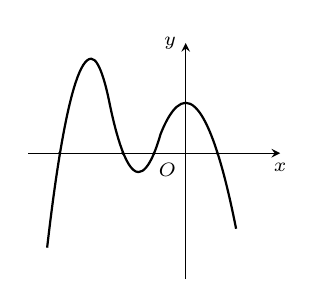
\begin{tikzpicture}[>=stealth,x=1.0cm,y=1.0cm,scale=0.4]
		\draw[color=gray,dash pattern=on 1pt off 1pt,xstep=1.0cm,ystep=1.0cm];
		\draw[->](-5,0)--(3,0) node[below] {\scriptsize $x$};
		\draw[->](0,-4)--(0,3.5) node[left] {\scriptsize $y$};
		\draw(0,0) node[below left] {\scriptsize $O$};
		\draw[thick,color=black](-4.4,-3) parabola bend(-3,3)(-2.4,1.5)
		(-2.4,1.5) parabola bend(-1.5,-.6) (-.8,.6)
		(-.8,.6) parabola bend(0,1.6) (1.6,-2.4);
		%\draw[dashed](-3,0)--(-3,2)--(0,2)(0,-2)--(1,-2)--(1,0)(3,0)--(3,-4)--(0,-4);
		\fill[black](-1,0) circle[radius=1.5pt](-2,0) circle[radius=1.5pt](-4,0) circle[radius=1.5pt]
		(1,0) circle[radius=1.5pt];
	\end{tikzpicture}}
	\loigiai{
		Đồ thị hàm số $f(x)$ cắt trục hoành tại $4$ điểm phân biệt có hoành độ $x_1$, $x_2$, $x_3$ ,$x_4$ (không mất tính tổng quát, giả sử $x_1<x_2<x_3<x_4$).\\
		Khi đó $f(x)=a\left(x-x_1\right)\left(x-x_2\right)\left(x-x_3\right)\left(x-x_4\right)$ và $a<0$.\\
		Ta có $f'(x)=f(x)\left[\dfrac{1}{\left(x-x_1\right)}+\dfrac{1}{\left(x-x_2\right)}+\dfrac{1}{\left(x-x_3\right)}+\dfrac{1}{\left(x-x_4\right)}\right]$\\
		nên $\dfrac{f'(x)}{f(x)}=\dfrac{1}{\left(x-x_1\right)}+\dfrac{1}{\left(x-x_2\right)}+\dfrac{1}{\left(x-x_3\right)}+\dfrac{1}{\left(x-x_4\right)}$.\\
		Lấy đạo hàm hai vế ta có
		\begin{center}
			$\left(\dfrac{f'(x)}{f(x)}\right)'=-\dfrac{1}{\left(x-x_1\right)^2}-\dfrac{1}{\left(x-x_2\right)^2}-\dfrac{1}{\left(x-x_3\right)^2}-\dfrac{1}{\left(x-x_4\right)^2}$ với $\forall x\in \mathbb{R}\setminus\left\{x_1;x_2;x_3;x_4 \right\}$.\\
			$\Rightarrow {f'}'(x)\cdot f(x)-\left[f'(x)\right]^2<0$ với $\forall x\in\left(-\infty;x_1\right)\cup\left(x_1;x_2\right)\cup\left(x_2;x_3\right)\cup\left(x_3;x_4\right)\cup\left(x_4;+\infty\right)$.\\
		\end{center}
		Mặt khác $2^x>0$ với $\forall x\in \mathbb{R}$.\\
		Vậy phương trình $f''(x)\cdot f(x)-\left[f'(x)\right]^2-2^x=0$ vô nghiệm.
	}
\end{ex}

%%==========Câu 50
\begin{ex}%[Dự án 15-TeamTeXHoa-Chuyên Lam Sơn Thanh Hóa-Hoàng Blue]%%[2D3G2-4]
	Cho hàm số $f(x)$ xác định và liên tục trên khoảng $(0;+\infty)$. Biết $\displaystyle\int\limits_2^3(x-1)^2\left[f(x-1)\right]^2\mathrm{d}x=\displaystyle\int\limits_1^2\dfrac{f(x)}{x}\mathrm{d}x=\dfrac{7}{24}$. Tính $\displaystyle\int\limits_1^2f(x)\mathrm{d}x$.
	\choice
	{$I=\dfrac{3}{7}$}
	{\True $I=\dfrac{3}{8}$}
	{$I=\dfrac{2}{7}$}
	{$I=\dfrac{7}{8}$}
	\loigiai{
		Đặt $t=x-1$ thì $\mathrm{d}t=\mathrm{d}x$.\\
		Đổi cận: $x=2 \Rightarrow t=1;x=3 \Rightarrow t=2$ nên\\
		$\displaystyle\int\limits_2^3(x-1)^2\left[f(x-1)\right]^2\mathrm{d}x=\displaystyle\int\limits_1^2t^2\left[f\left(t\right)\right]^2\mathrm{d}t=\displaystyle\int\limits_1^2x^2\left[f(x)\right]^2\mathrm{d}x=\dfrac{7}{24}$.\\
		Ta có $\displaystyle\int\limits_1^2\dfrac{f(x)}{x}\mathrm{d}x=\displaystyle\int\limits_1^2xf(x)\dfrac{1}{x^2}\mathrm{d}x=\dfrac{7}{24}$
		và $\displaystyle\int\limits_1^2\dfrac{1}{x^4}\mathrm{d}x=\dfrac{7}{24}$.\\
		Từ đó ta được $\displaystyle\int\limits_1^2x^2\left[f(x)\right]^2\mathrm{d}x-2\displaystyle\int\limits_1^2xf(x)\dfrac{1}{x^2}\mathrm{d}x+\displaystyle\int\limits_1^2\dfrac{1}{x^4}\mathrm{d}x=0$.\\
		Hay $\displaystyle\int\limits_1^2\left(x^2\left[f(x)\right]^2-2xf(x)\dfrac{1}{x^2}+\dfrac{1}{x^4}\right)\mathrm{d}x=0 \Leftrightarrow \displaystyle\int\limits_1^2\left(xf(x)-\dfrac{1}{x^2}\right)^2\mathrm{d}x=0$.\\
		Từ đó suy ra $xf(x)-\dfrac{1}{x^2}=0 \, , \forall x \in [1;2] \Leftrightarrow f(x)=\dfrac{1}{x^3}$.\\
		Vậy $\displaystyle\int\limits_1^2f(x)\mathrm{d}x=\displaystyle\int\limits_1^2\dfrac{1}{x^3} \mathrm{d}x=\dfrac{3}{8}$.}
\end{ex}
\Closesolutionfile{ans}